%%%%%%%%%%%%%%%%%%%%%%%%%%%%%%%%%%%%%%%%%%%%%%%%%%%%%%%%%%%%%%%%%%%%%%%%%%%%%%%%%%%%%%%%%%%%%%%%%%%%%%%%%%%%%%%%%%%%%%%%%%%%%%%%%%%%%%%%%%%%%%%%%%%%%%%%%%%
% This is just an example/guide for you to refer to when producing your supplementary material for your Frontiers article.                                 %
%%%%%%%%%%%%%%%%%%%%%%%%%%%%%%%%%%%%%%%%%%%%%%%%%%%%%%%%%%%%%%%%%%%%%%%%%%%%%%%%%%%%%%%%%%%%%%%%%%%%%%%%%%%%%%%%%%%%%%%%%%%%%%%%%%%%%%%%%%%%%%%%%%%%%%%%%%%

%%% Version 2.5 Generated 2018/06/15 %%%
%%% You will need to have the following packages installed: datetime, fmtcount, etoolbox, fcprefix, which are normally inlcuded in WinEdt. %%%
%%% In http://www.ctan.org/ you can find the packages and how to install them, if necessary. %%%
%%%  NB logo1.jpg is required in the path in order to correctly compile front page header %%%

\documentclass[utf8]{frontiers_suppmat} % for all articles
\usepackage{url,hyperref,lineno,microtype}
\usepackage[onehalfspacing]{setspace}



% Leave a blank line between paragraphs instead of using \\

\begin{document}
\onecolumn
\firstpage{1}

\title[Supplementary Material]{{\helveticaitalic{Supplementary Material}}:
\\ \helvetica{A dynamic optimality principle for water use strategies explains isohydric to anisohydric plant responses to drought}} %Please insert the title of your article here


\maketitle


\clearpage

\section{Supplementary Tables and Figures}

\subsection{Figures}

\begin{figure}[b]
    \centering
    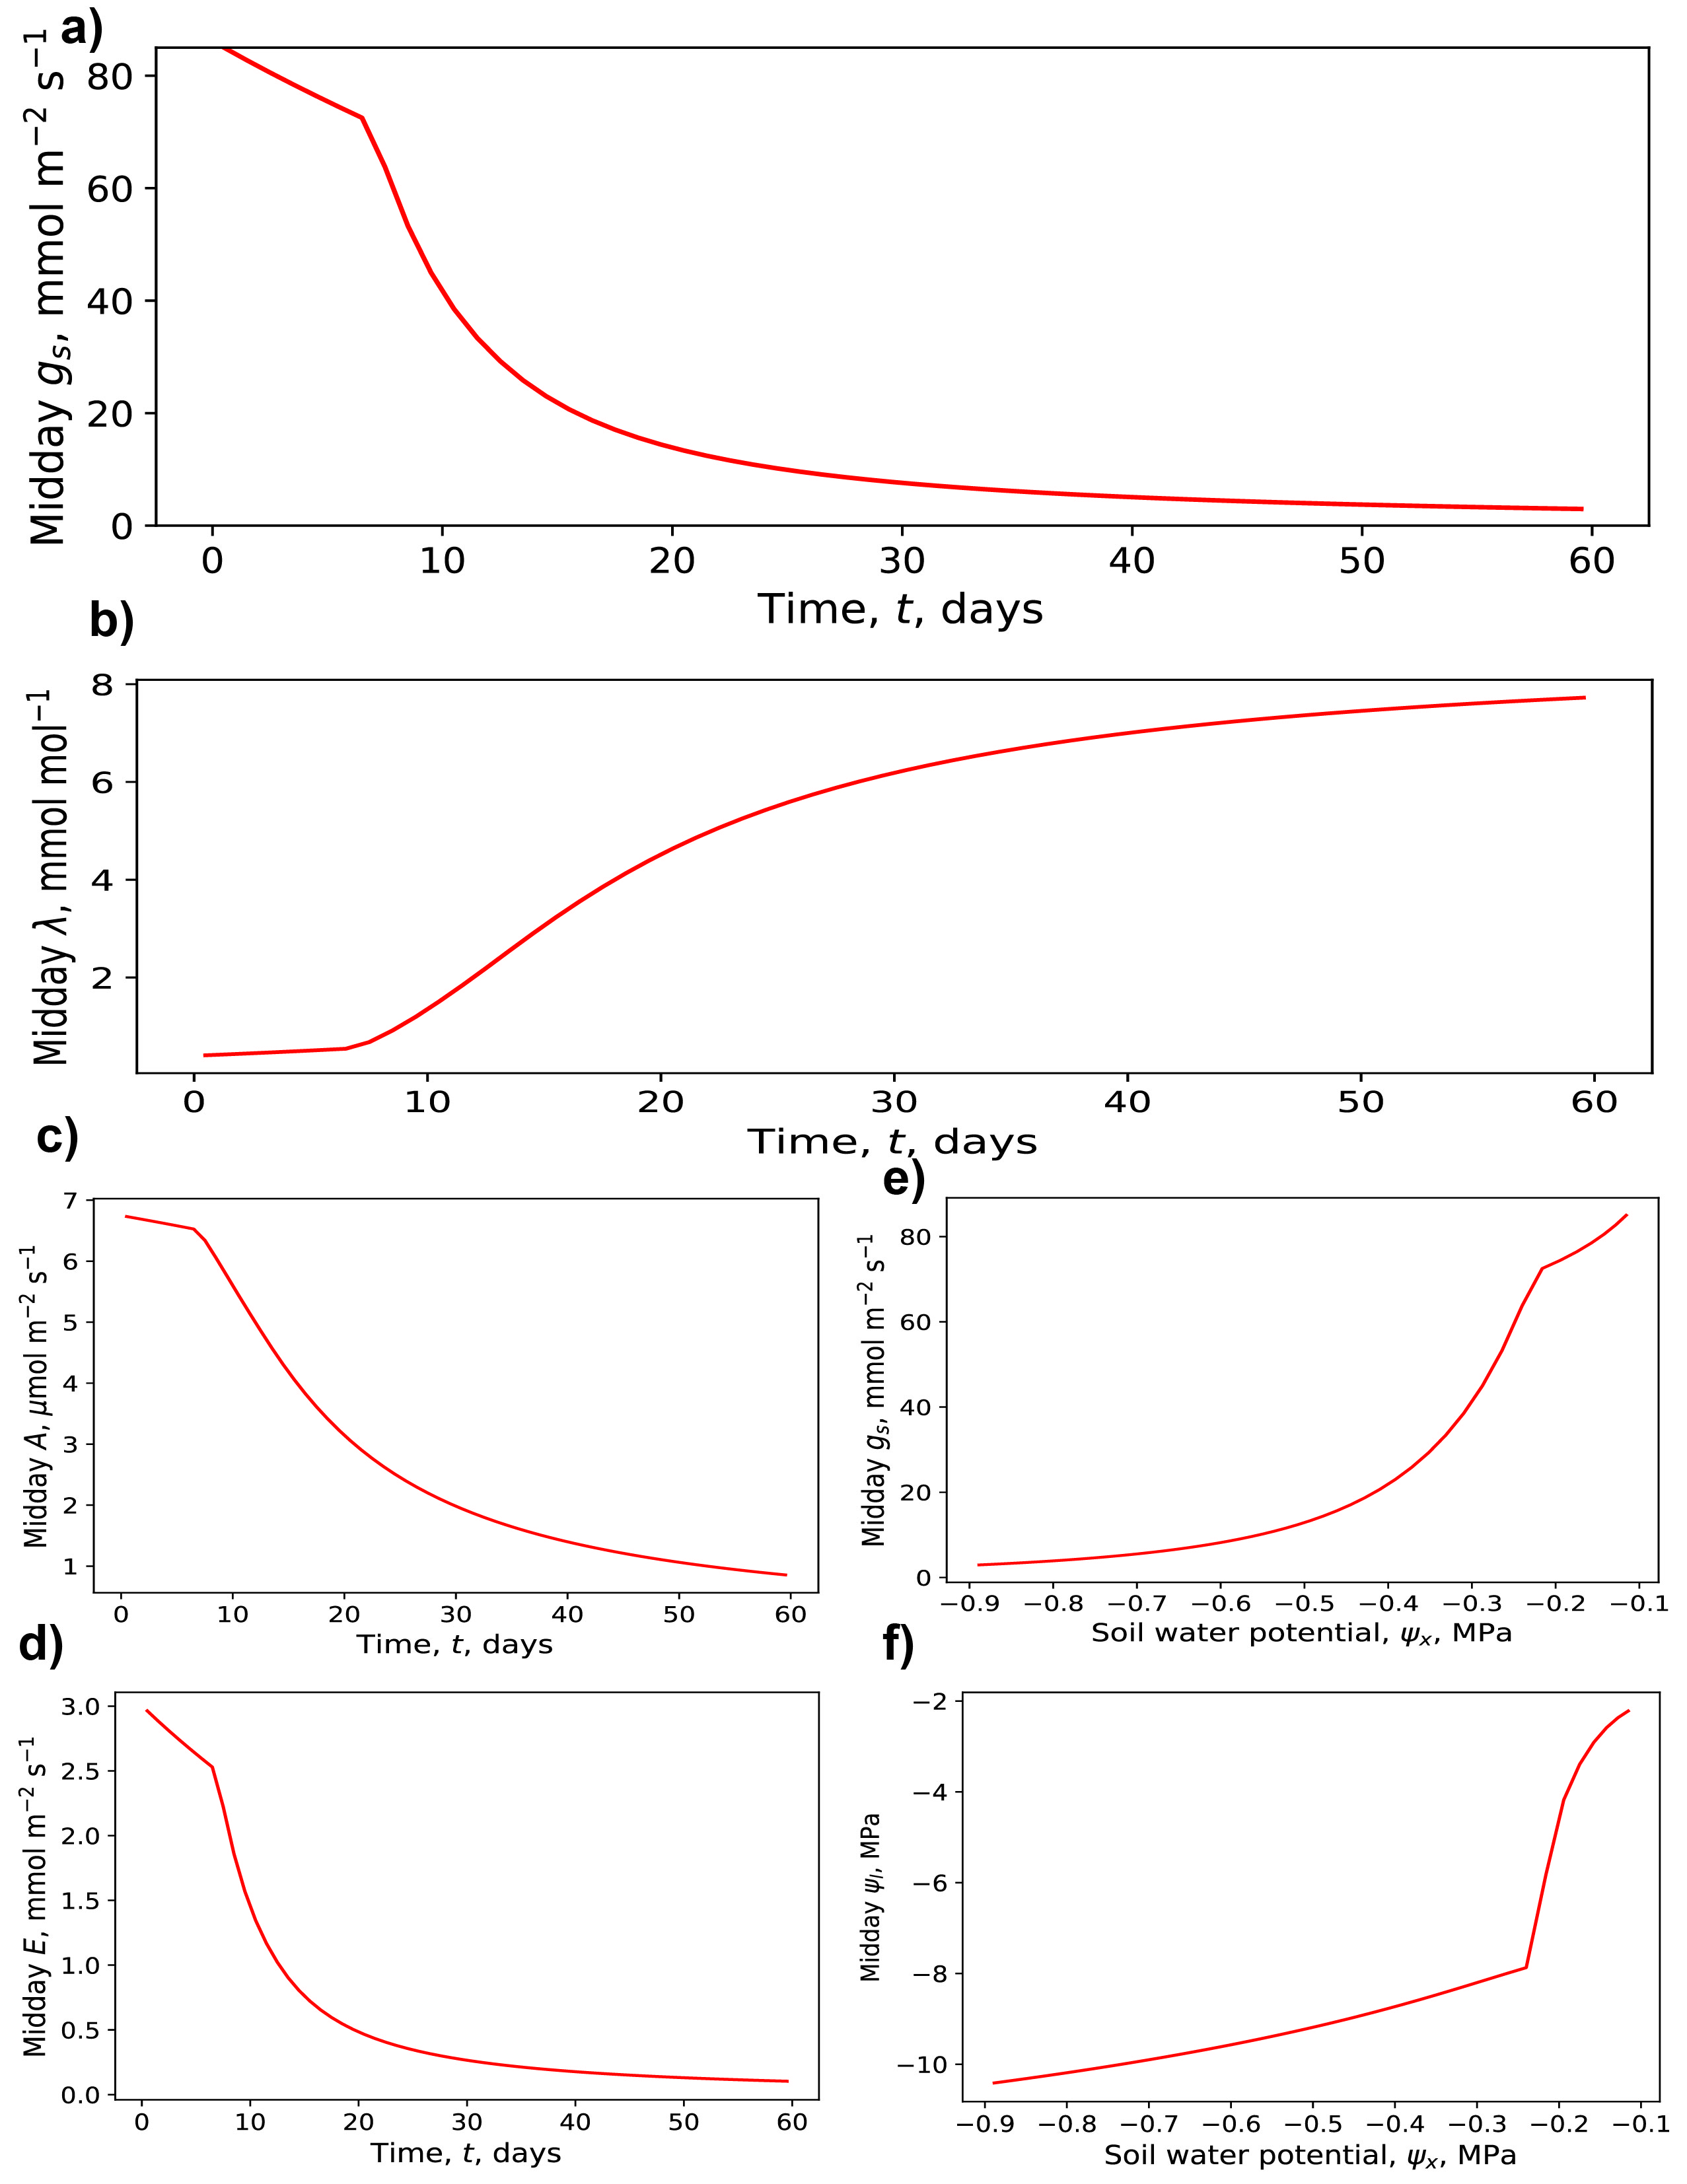
\includegraphics[scale=0.15]{Long_Drought_Fig.jpg}
    \caption{Results of a 60-day drought simulation where at time $t=0$, soil moisture $x(0) =0.25$ for the gradual and resistant VC (figure 2 of the main text). The terminal marginal water use efficiency is set at $\lambda(60) = 1$ mmol mol$^{-1}$. Other parameters have the same values as those in table 1 in the main text except $Z_r = 1$m. The competitive water sinks are soil free drainage and competing plants with similar vulnerability curves (VCs) and water use strategy (WUS) to those modeled. The competing plants have access to only 20\% of the root zone water of each modeled plant. a) Midday trends of stomatal conductance ($g_s$) with $t$ and b) midday $\lambda$ with $t$. c) Midday carbon assimilation rate ($A$) and d) midday transpiration rate ($E$) with $t$. e) Midday $g_s$ and f) midday leaf water potential $\psi_l$ with soil water potential $\psi_x$.}
    \label{fig:Drought}
\end{figure}

\begin{figure}[b]
    \centering
    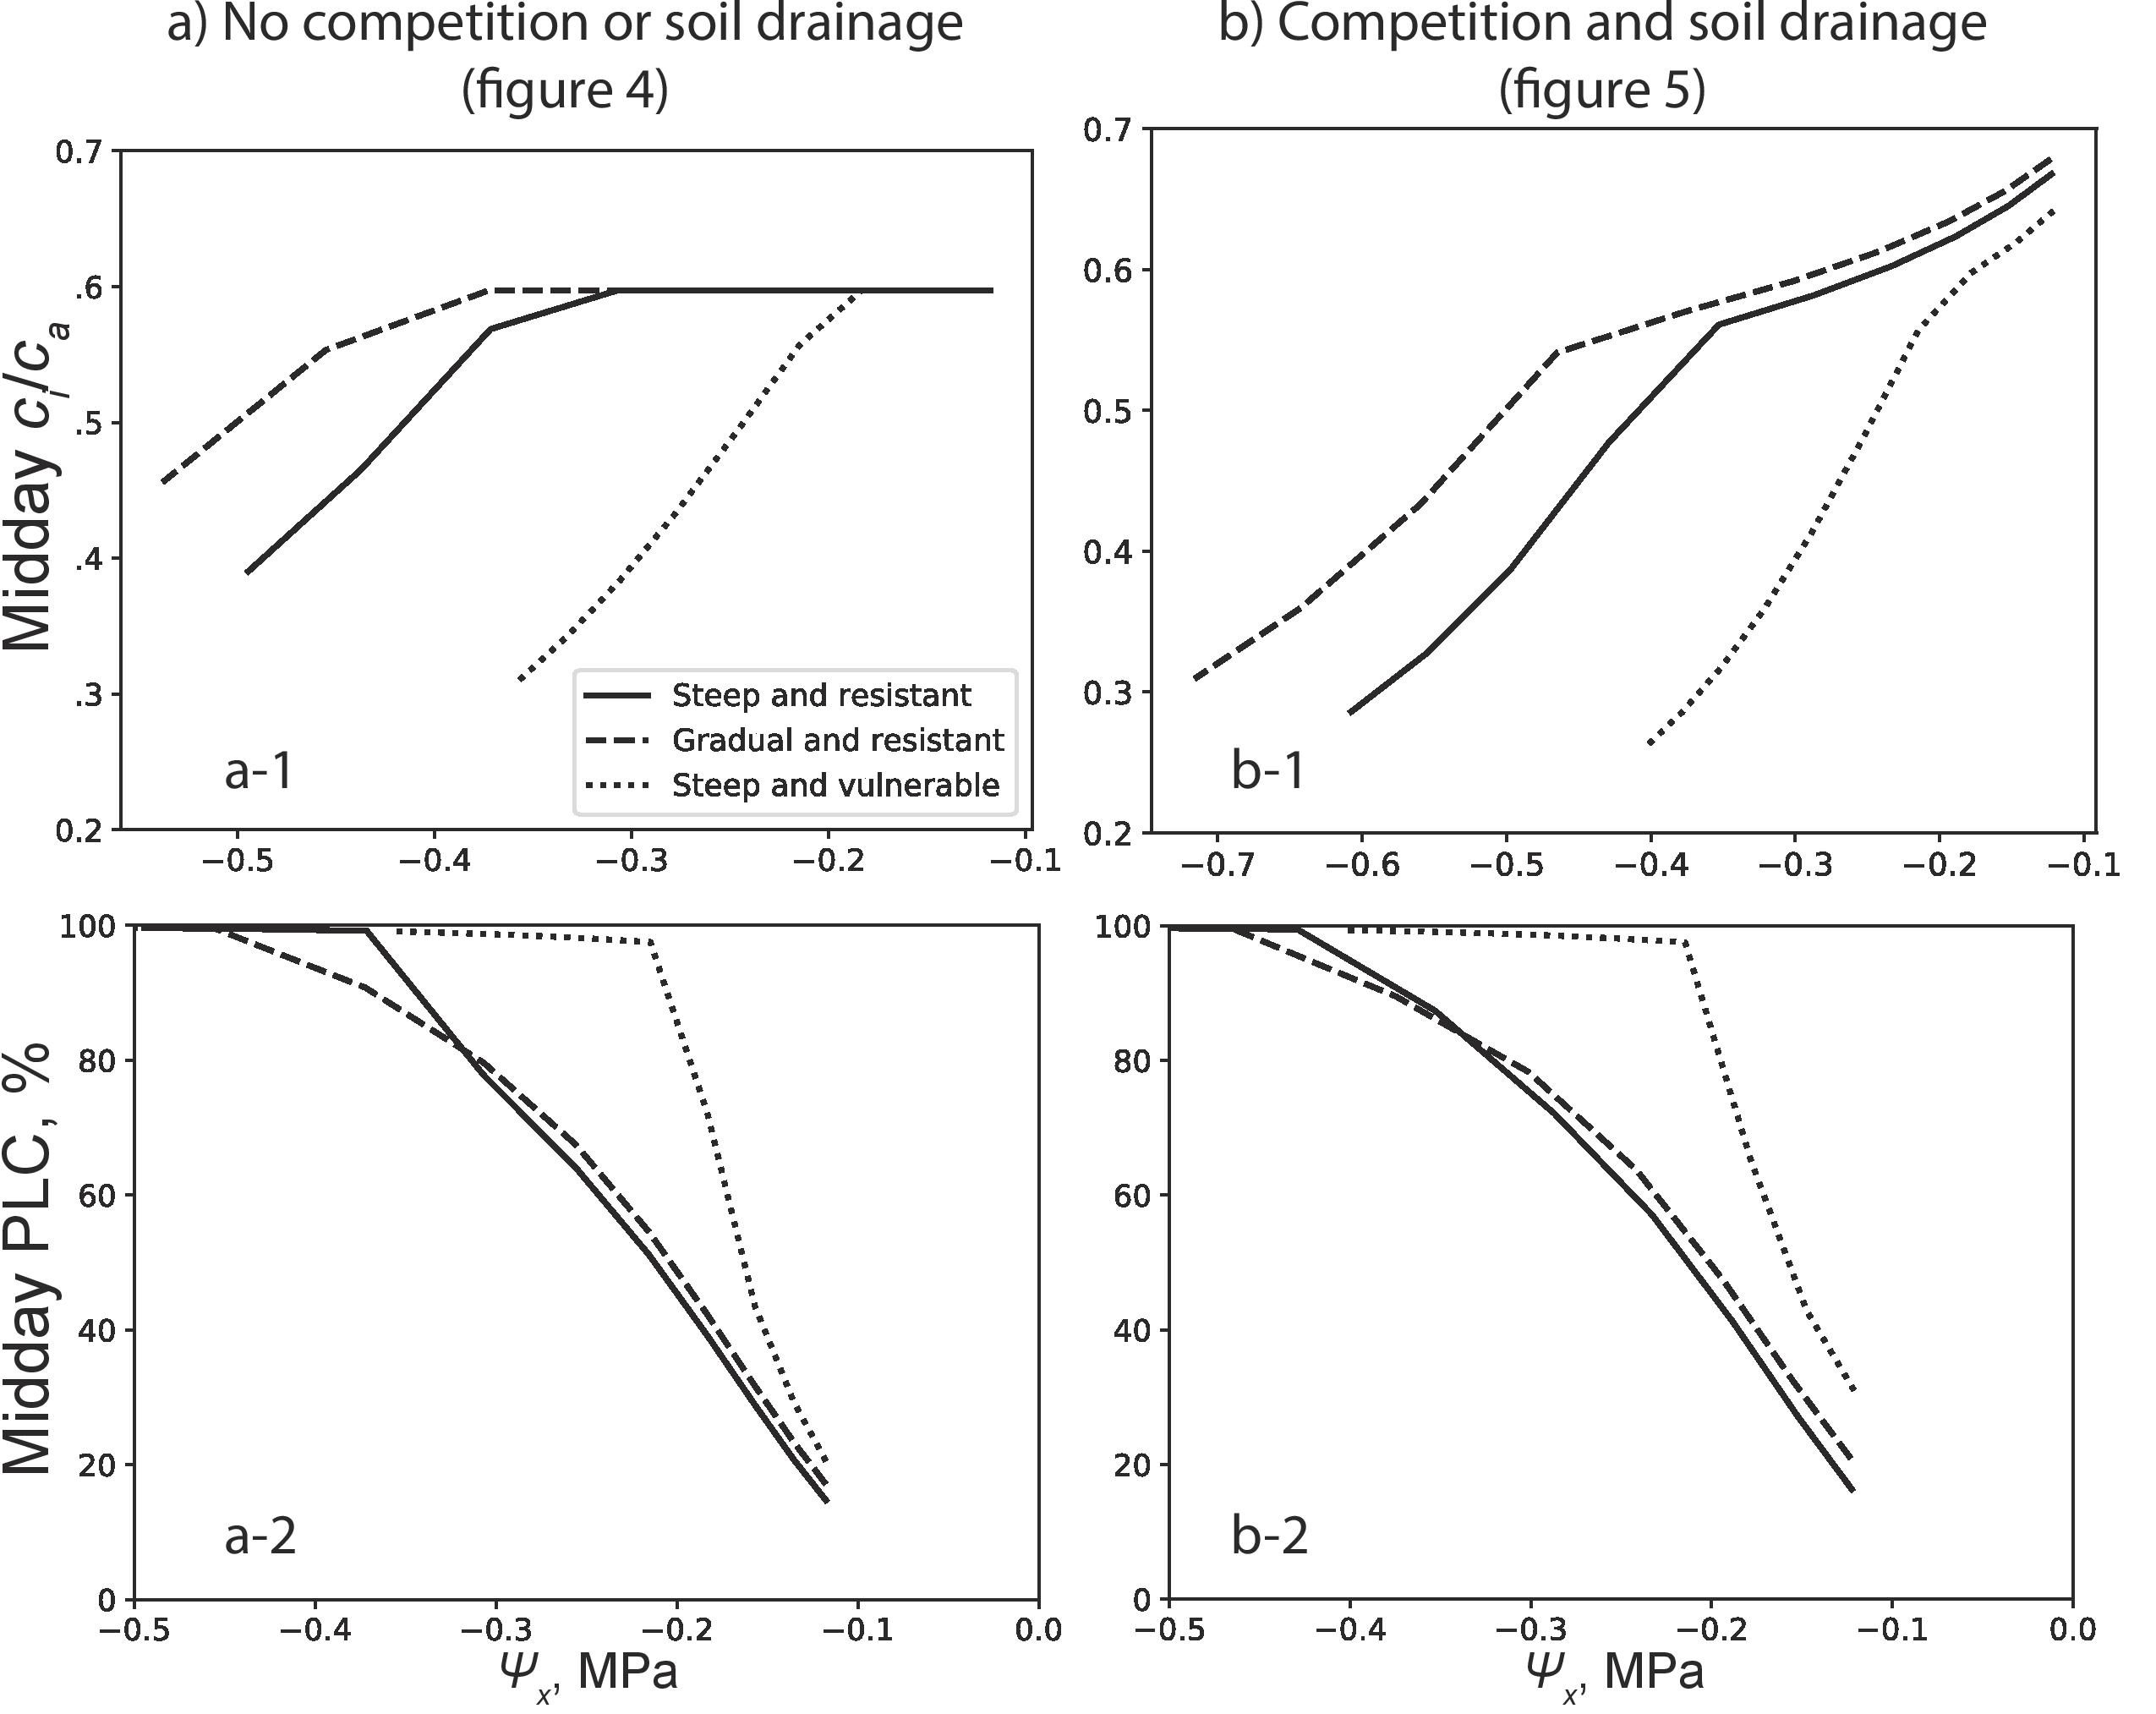
\includegraphics[scale=0.75]{PLC_cica.jpg}
    \caption{Trends of a-1,b-1) midday ratio of internal to atmospheric carbon concentration $c_i / c_a$ and of a-2,b-2) midday percent loss of conductance (PLC) of the combined soil-root-stem-leaf continuum with soil water potential $\psi_x$. Panel A refers to the simulation shown in figure 4 of the main text where no competition or soil drainage was present. Panel B refers to the simulation shown in figure 5 of the main text where both competition and soil drainage were present. These results also compare the three different vulnerability curves (VCs) plotted in figure 2 of the main text.}
    \label{fig:PLC_cica}
\end{figure}
% All supplementary files are deposited to FigShare for permanent storage during the production stage of the article and receive a DOI. For more information on Supplementary Material and for details on the different file types accepted, please see \href{http://home.frontiersin.org/about/author-guidelines#SupplementaryMaterial}{the Supplementary Material section} of the Author Guidelines.

% Figures, tables, and images will be published under a Creative Commons CC-BY licence and permission must be obtained for use of copyrighted material from other sources (including re-published/adapted/modified/partial figures and images from the internet). It is the responsibility of the authors to acquire the licenses, to follow any citation instructions requested by third-party rights holders, and cover any supplementary charges.

%% Figures, tables, and images will be published under a Creative Commons CC-BY licence and permission must be obtained for use of copyrighted material from other sources (including re-published/adapted/modified/partial figures and images from the internet). It is the responsibility of the authors to acquire the licenses, to follow any citation instructions requested by third-party rights holders, and cover any supplementary charges.



%%% There is no need for adding the file termination, as long as you indicate where the file is saved. In the examples below the files (logo1.eps and logos.eps) are in the Frontiers LaTeX folder
%%% If using *.tif files convert them to .jpg or .png
%%%  NB logo1.eps is required in the path in order to correctly compile front page header %%%


%%% If you are submitting a figure with subfigures please combine these into one image file with part labels integrated.
%%% If you don't add the figures in the LaTeX files, please upload them when submitting the article.
%%% Frontiers will add the figures at the end of the provisional pdf automatically
%%% The use of LaTeX coding to draw Diagrams/Figures/Structures should be avoided. They should be external callouts including graphics.


%\bibliographystyle{frontiersinSCNS_ENG_HUMS} %  for Science, Engineering and Humanities and Social Sciences articles, for Humanities and Social Sciences articles please include page numbers in the in-text citations
%\bibliographystyle{frontiersinHLTH&FPHY} % for Health and Physics articles
%\bibliography{test}

\end{document}
